\section{Control Method} \label{sec:control_method}

In this section we combine sampling, barrier functions and energy tank into a novel model-based control framework for robust and safe interaction control. We use the presented sampling method to generate joint velocity command sequences that optimize a task-dependent objective in a receding horizon fashion. We encode a set of tasks and safety related objectives as different cost terms. Nevertheless, sampling does not inherently provide guarantees and therefore we need a method to enhance safety. We address this problem using ZBFs as a non-invasive way to change the command sequence when constraints are not fulfilled. In particular, we solve an optimization problem that ensure foward invariance with respect to the safe set when joint velocities are accurately tracked. While the safety objectives are here formulated on a kinematic level (obstacle avoidance, joint and cartesian limits), we are also interested to the robustness of the dynamical system during interaction, especially in case of unexpected events that could compromise its stability. For this purpose, we complete the proposed framework with a passivity analysis and use an energy tank to bound the energy dissipated during the manipulation task. Passivity is guaranteed in the form of an additional constraint in the quadratic program which naturally fits the other algorithmic components. Finally we present different implementation alternatives taking into account that sampling takes often more time then the quadratic program and therefore a multi-rate cascaded control architecture might be needed. 

\subsection{Sampling-based control}
The sampling-based framework offers the freedom to directly plan in torque space or use position/velocity control and defer tracking to a low-level controller. In fact, directly planning in the joint space allows us to account for objectives which are not in the operational control space such as joint limits and self-collision avoidance. The internal model used to sample trajectory rollouts has the same form as in \eqref{eq:eom}. Joint velocity commands are sampled and then translated to motor torques:
\begin{equation}
    \vect{\tau}_{cmd} = \matr{K}_{D} (\command - \dconfigRobot) + \robotCoriolis,
\end{equation}
with an appropriate choice of the positive-definite diagonal gain matrix $\matr{K}_{D} \in \nR{\robotDoF\times\robotDoF}$. 

\subsection{Cost shaping}
As described in Section~\ref{sec:formulation}, the control objective is to drive the system to a desired state. Furthermore, as state constraints are not explicitly taken into account by the formulation, a common heuristic is to penalize deviations from feasible states in the cost function. Input constraints are easier to handle as the non-linear dynamics can be augmented with a function that projects the sampled inputs to the feasible set $\mathcal{U}$. In the following we define several cost components associated with the different high-level objectives and constraints.
We denote by $\mathds{1}[\cdot]$ the \textit{indicator function} such that,
\begin{equation}
    \mathds{1}[x] = 
    \begin{cases}
    1 & \text{if } x \text{ is True} \\
    0 & \text{otherwise}.
    \end{cases}
\end{equation}
In the following we drop from the notation the dependence on the current state. We use $\weightMatrix{}$ to denote positive semidefinite weight matrices and $\weightScalar{}$ for non-negative scalar parameters. 

\paragraph{Target reaching} in the target reaching task, the goal is to bring a frame attached to the robot (generally the end-effector frame) to a desired pose. We define with $\matr{T}$ and $\matr{T}^*$ the current and desired target frame pose, respectively. The \textit{tracking cost} is computed as a weighted distance in the tangent space to $SE(3)$ using the logarithmic mapping~\cite{blanco2010tutorial}:
\begin{equation} \label{eq:tracking_cost}
     c_{t} = || \log(\matr{T} - \matr{T}^{*}) ||^2_{\weightMatrix{t}}.
 \end{equation}
 
 \paragraph{Collision avoidance} let $\contact \in \{0, 1\}$ represent an auxiliary variable which is equal to 1 when the manipulator is in contact with the environment. The value of $\contact$ can be computed searching for collisions between bodies. 
 $\contact$ is used to avoid collisions during contact-free motions of the end-effector. 
 The \textit{contact cost} is defined as,
 \begin{equation}
     c_{\contact}= \weightScalar{\contact} \contact(\state).
 \end{equation}

 \paragraph{Joint position limits} the manipulator is subject to physical joint limits. These can be addressed by introducing a cost component that penalizes violation of the constraints. We define the \textit{joint limits cost} with:
 \begin{align}
     &c_{j} = \mathds{1}[\configRobot > \upperLimits](\weightScalar{j} + ||\upperLimits - \configRobot||^2_{\weightMatrix{js}}) + \nonumber\\ 
     &\qquad\mathds{1}[\configRobot < \lowerLimits](\weightScalar{j} +  || \configRobot - \lowerLimits||^2_{\weightMatrix{js}}), 
 \end{align}
 where the scalar $\weightScalar{j}$ is a constant cost added when the limit is violated. The matrix $\weightMatrix{js}$ adds a quadratic term in the limit violation. This was shown in~\cite{williams_information-theoretic_2018} to help the controller find its way back if poor sampling brings the system outside of the joint position limits.
 
 \paragraph{Arm reach} we introduce an additional term that penalizes configurations where the arm's end-effector moves excessively far from the base. This helps to bias solutions where base motion is preferred over stretching the arm which can lead to singular configurations. The translation vector from the end-effector frame $\mathcal{E}$ to the arm base frame $\mathcal{B}$ is defined with the vector $\vect{p}_{BE} \in \nR{3}$. The current reach is then $r_{\text{curr}} = || \vect{p}_{BE} ||^2$. Given a maximum reach $r_{\text{max}} \in \nR{}_{\geq 0}$, the \textit{reach cost} is then defined by:
 \begin{equation}
   c_r = \mathds{1}[r_{\text{curr}} > r_{\text{max}}] (\weightScalar{r} + \weightScalar{rs}(r_{\text{curr}} - r_{\text{max}})^2).    
 \end{equation}

 \paragraph{Self-collision avoidance} similarly to arm reach, self-collision avoidance can be implemented as an additional cost term which is active when the distance between a pair of frames is less than a pair-dependent threshold. Given the distance between two frames $d_{ij}$ and a threshold $d^{min}_{ij}$ the self-collision cost for the pair is:
 \begin{equation}
   c_{sc} = \sum_{ij, i \neq j} \mathds{1}[d_{ij} < d^{min}_{ij}] (\weightScalar{r} + \weightScalar{rs}(d^{min}_{ij} - d_{ij})^2).    
 \end{equation}
 
 \paragraph{Object manipulation} in the manipulation task the goal is to change the state of an articulated object through interaction. The \textit{manipulation cost} penalizes deviations from the target object configuration $\configObject^{*}$,
\begin{equation}
    c_o(\configObject; \weightMatrix{o}) = || \configObject - \configObject^{*}||^2_{\weightMatrix{o}}.
\end{equation}
\paragraph{Power minimization} we propose a new cost component that takes into account the power dissipated to perform the task. In fact a successful interaction (i.e opening the door) could happen in multiple ways, however trajectories that dissipate low power are most efficient as they do not act against the environment and robot kinematic constraints. We leverage the fact that as rollouts are performed in simulation, the joint torque generated through interaction can be easily computed by summing the contribution of each force $\vect{f}_c \in \nR{3}$ at each contact point $c$:
\begin{equation}
\boldsymbol{\tau}_{ext} = \sum\limits_{c} \matr{J}_c \vect{f}_c,    
\end{equation}
where $\matr{J}_c$ is the contact Jacobian. The power dissipated during the task is therefore $-\boldsymbol{\tau}_{ext}^T\command$, which is positive when acting ``against" the environment. The cost associated with power penalization is:
\begin{equation}
   c_p = \weightScalar{p} \cdot \max(0, - \boldsymbol{\tau}_{ext}^T\command - p_{max}),      
 \end{equation}
where $p_{max}$ is the maximum power that can be dissipated during the task.
As we will later see, this is the power that is drained from the tank and therefore, this cost component has the additional benefit of helping to avoid depletion of the energy tank.

\subsection{Cost scheduling}
The manipulation task consists of two phases. In a first phase the manipulator reaches an estimated contact point, allowing for a fast and successful exploration in the following interaction phase. In the second phase, the goal is to bring the object to the desired state while keeping the end-effector close to the contact location. This switch is enabled by turning on the object manipulation cost $c_o$. Reducing the end-effector position penalty during the manipulation phase allows the controller to choose a trajectory that fully exploits the contact dynamics by changing the hand pose. 

%This approach is in contrast with previous works where manipulation generally follows a prescribed grasping state~\cite{abraham_model-based_2020}. Grasping introduces a kinematic constraint that, while reducing the optimal control search space, does not allow for more flexible, contact-based behaviors to emerge such as pulling, pushing or sliding. 

\subsection{Barrier Functions}
In the previous subsection a combination of cost components were introduced in order to address both performance and safety. The variety of objectives makes the cost landscape highly complex such that trading off performance against safety objectives can be quite challenging and tedious. Furthermore, sampling does not provide any formal guarantee that constraints encoded in the form of additional cost terms will be satisfied. In the following, we look at how barrier functions can encode safety-critical constraints. We start by deriving the ZBF constraints based on the differential kinematics equation,
\begin{equation}
    \dot{\state} = \matr{J} \dconfigRobot\;.
\end{equation}
As described in \cite{benzi2021optimization}, a simple ZBF can be derived for each joint to keep it between its lower and upper bounds, $q_i^-$ and $q_i^+$, respectively:
\begin{equation}
h_{ql}^i = \frac{(q_i^+ - q)(q - q_i^-)}{(q_i^+ - q_i^-)}\;.
\end{equation}
In the following we treat the safety requirements associated to robot frames and denote with $\vect{p}_{i} \in \nR{3}$ the position of frame $i$ computed through forward kinematics.  
The self-collision safe set can be obtained by approximating potentially colliding frames with non-intersecting spheres. Then the self-collision ZBF is defined as,
\begin{equation}
    h_{sc}^{ij} = \frac{1}{2}(||\vect{p}_i - \vect{p}_j||^2 - d_c^2),
\end{equation}
where $d_c = r_i + r_j$ is the sum of the radius of the two collision spheres associated with the $i$\textsuperscript{th}  and $j$\textsuperscript{th} collision pair frames. Note that we can similarly encode arm reach limits. In fact, the following is a valid ZBF, positive only when the end-effector is within the prescribed reach with respect to the arm base,
\begin{equation}
    h_{ar} = \frac{1}{2}(D_r^2 - (\vect{p}_{ee} - \vect{p}_{base})^T P (\vect{p}_{ee} - \vect{p}_{base}) ).
\end{equation}
The projection matrix $P = \text{diag}(1, 1, 0) \in \nR{3 \times 3}$ makes sure that the reach is only computed in the 2D plane. This prevents the arm to stretch out and reach singular configurations that are hard to escape. Each of these ZBFs translates to a constraint of the form in \eqref{eq:cbf-const} which is affine in the commands. 

\subsection{Energy Tank}
As described in \sect \ref{sec:theory}, energy tanks can be used to \emph{passify} the system and ensuring so stability. Inspired by the work in \cite{benzi2021optimization} and \cite{shahriari2018valve}, this adaptation naturally fits the control method we have developed so far. After the system model is augmented with a virtual tank, we are left with the task of defining the \emph{power ports} connected to the tank that ensure passivity is preserved. To this end, we perform a passivity analysis of the \emph{real} system. Its 
velocity controller follows a dynamically compensated PI control law:
\begin{equation}
\commandTorque = \coriolis \dconfigRobotDesired + g(\configRobot) - \matr{K}_D \dconfigRobotError - \matr{K}_I \int_{0}^{\sigma} \dconfigRobotError\ dt,
\end{equation}
with the auxiliary error variable $\configRobotError =  \configRobot - \configRobotDesired$. We define the system energy as, 
\begin{equation}
    S_{robot} = \frac{1}{2} \dconfigRobotError^T \massMatrix \dconfigRobotError + \frac{1}{2} \configRobotError^T \matr{K}_P \configRobotError.
\end{equation}
In order to study the passivity of the system, we need to derive the robot energy dynamics. A complete derivation can be found in the Appendix~\ref{app:passivity_analysis}. It turns out that:
\begin{equation}
    \dot{S}_{robot} = \dconfigRobotError^T \externalTorque - \dconfigRobotError^T \matr{K}_D \dconfigRobotError \leq \dconfigRobotError^T \externalTorque. 
\end{equation}
The power flow through the external torque has indefinite sign and can lead to a loss of passivity. Since the environment is passive, there exists an environment energy such that~\cite{shahriari2018valve},
\begin{equation}
    \dot{S}_{env} \leq -\dconfigRobot^T \externalTorque.
\end{equation}
The energy tank is finally connected to the system through the power port $(\dconfigRobot^*, \externalTorque)$ and therefore,
\begin{equation} \label{eq:tank_dynamics}
\dot{S}_{tank} = \dconfigRobot^{*T} \externalTorque. 
\end{equation}
The time evolution of the autonomous system's energy is,
\begin{equation}
\begin{aligned}
    \dot{S}_{tot} &= \dot{S}_{robot} + \dot{S}_{tank} + \dot{S}_{env} \\
    &\leq \dconfigRobotError^T \externalTorque + \dconfigRobot^{*T} \externalTorque - \dconfigRobot^T \externalTorque \leq 0,
\end{aligned}
\end{equation}
showing the system's passivity. The increase of the robot's energy is compensated by a reduction of the tank's energy. Passivity is ensured if,
\begin{equation}
    \int_{0}^{\sigma} \boldsymbol{\tau}_{ext}^T \command \ dt \geq \epsilon,
\end{equation}
where $\epsilon$ is a positive minimum residual energy to avoid a singularity condition and complete tank depletion.

\subsection{Closing the loop}
As described in \sect \ref{sec:theory}, we can formulate a quadratic program to find the command which is the closest to the sampled one while also satisfying the ZBF and passivity constraints previously introduced:
\begin{mini}|s| 
{\tilde{\vect{u}}_t, \boldsymbol{\delta}}{||\tilde{\vect{u}}_t - \command_t||^2 + \boldsymbol{\delta}^T \matr{P} \boldsymbol{\delta}\quad \text{(FILTER-QP)}}{}{\label{eq:cbf-qp}}
\addConstraint{\dot{h}^i_{ql} \geq -{h}_{ql} + \delta^i_{ql} \quad \forall \ i \in [1,  m] }{}{\quad \text{(Joint Limits)}}
\addConstraint{\dot{h}^{ij}_{sc} \geq -{h}_{ij} + \delta^{ij}_{sc} \quad \forall \ (i,j) \in \mathcal{I}}{}{\quad \text{(Self Collision)}}
\addConstraint{\dot{h}^i_{ar} \geq -{h}_{ar} + \delta^i_{ar}}{}{\quad \text{(Arm Reach)}}
\addConstraint{\int_{0}^{\sigma} \boldsymbol{\tau}_{ext}^T \command \ dt \geq -S(x_t(0)) + \epsilon + \delta_t}{}{\quad \text{(Passivity)}}
\addConstraint{\tilde{\vect{u}}_t \in \mathcal{U}}{}{\quad \text{(Input Limits)}},
\end{mini}
where $\boldsymbol{\delta}$ is the vector of slack variables and $\matr{P}$ is a positive definite diagonal matrix. Finally, the set denoted by $\mathcal{I}$ is the set of collision link pairs.  We name this problem FILTER-QP as it changes the control input only if it is unsafe or causes a loss of passivity. Instead of simply applying this optimization point-wise, we \emph{filter} the full input sequence in a sequential manner. After a policy update and for each time step, a FILTER-QP is solved. The newly computed command is applied to advance to the next step in the horizon as shown in \algo \ref{algo:sequential_qp}. The resulting filtered input sequence $\bar{U}^*_t$ is then used to warm-start the nominal policy for the next round of rollout sampling (see \fig \ref{fig:receding_horizon}). 

\begin{algorithm}
\caption{Sequential FILTER-QP \label{algo:sequential_qp}}
\KwData{optimal input sequence $U^*_t = \{ \command^*_t, \dots, \command^*_{t+T-1}\} = \{\boldsymbol{\mu}_t, \dots, \boldsymbol{\mu}_{t+T-1}\}$ , current state $\vect{x}_t$, 
tank state $x_t$}
\KwResult{filtered input trajectory $\bar{U}^*_t$}
$\vect{x} \gets \vect{x}_t$\;
$\command \gets \command^*_t$\;
$n \gets 0$\;
\While{$n < T$}{
  $\bar{\command}_{t+n} \gets \text{FILTER-QP}(\vect{x}, \command, x_t, \boldsymbol{\tau}_{ext})$ \hfill (\eqn \ref{eq:cbf-qp}) \\
  $\vect{x}, \boldsymbol{\tau}_{ext} \gets $Step Simulation \hfill (\eqn \ref{eq:eom})\\
  $x_t \gets$ Integrate Tank \hfill (\eqn \ref{eq:tank_dynamics}) \\
  $\command \gets {\command}^*_{t+n+1}$ \\
  $n = n + 1$
}
\end{algorithm}

\subsection{Cascaded control architecture}
The expensive rollout sampling procedure often limits the rate of the controller. Instead, the QP can be efficiently solved at almost the same rate as the low-level controller. We propose a \emph{cascaded control} architecture composed of a low-rate policy update block and a high-rate low-level control loop. The latter solves the FILTER-QP in \eqref{eq:cbf-qp} point-wise to find the best input according to the latest received measurements. The full cascaded control architecture is shown in \fig \ref{fig:cascaded_architecture}.

\begin{figure}[t!]
\centering
\hspace*{-0.7cm}
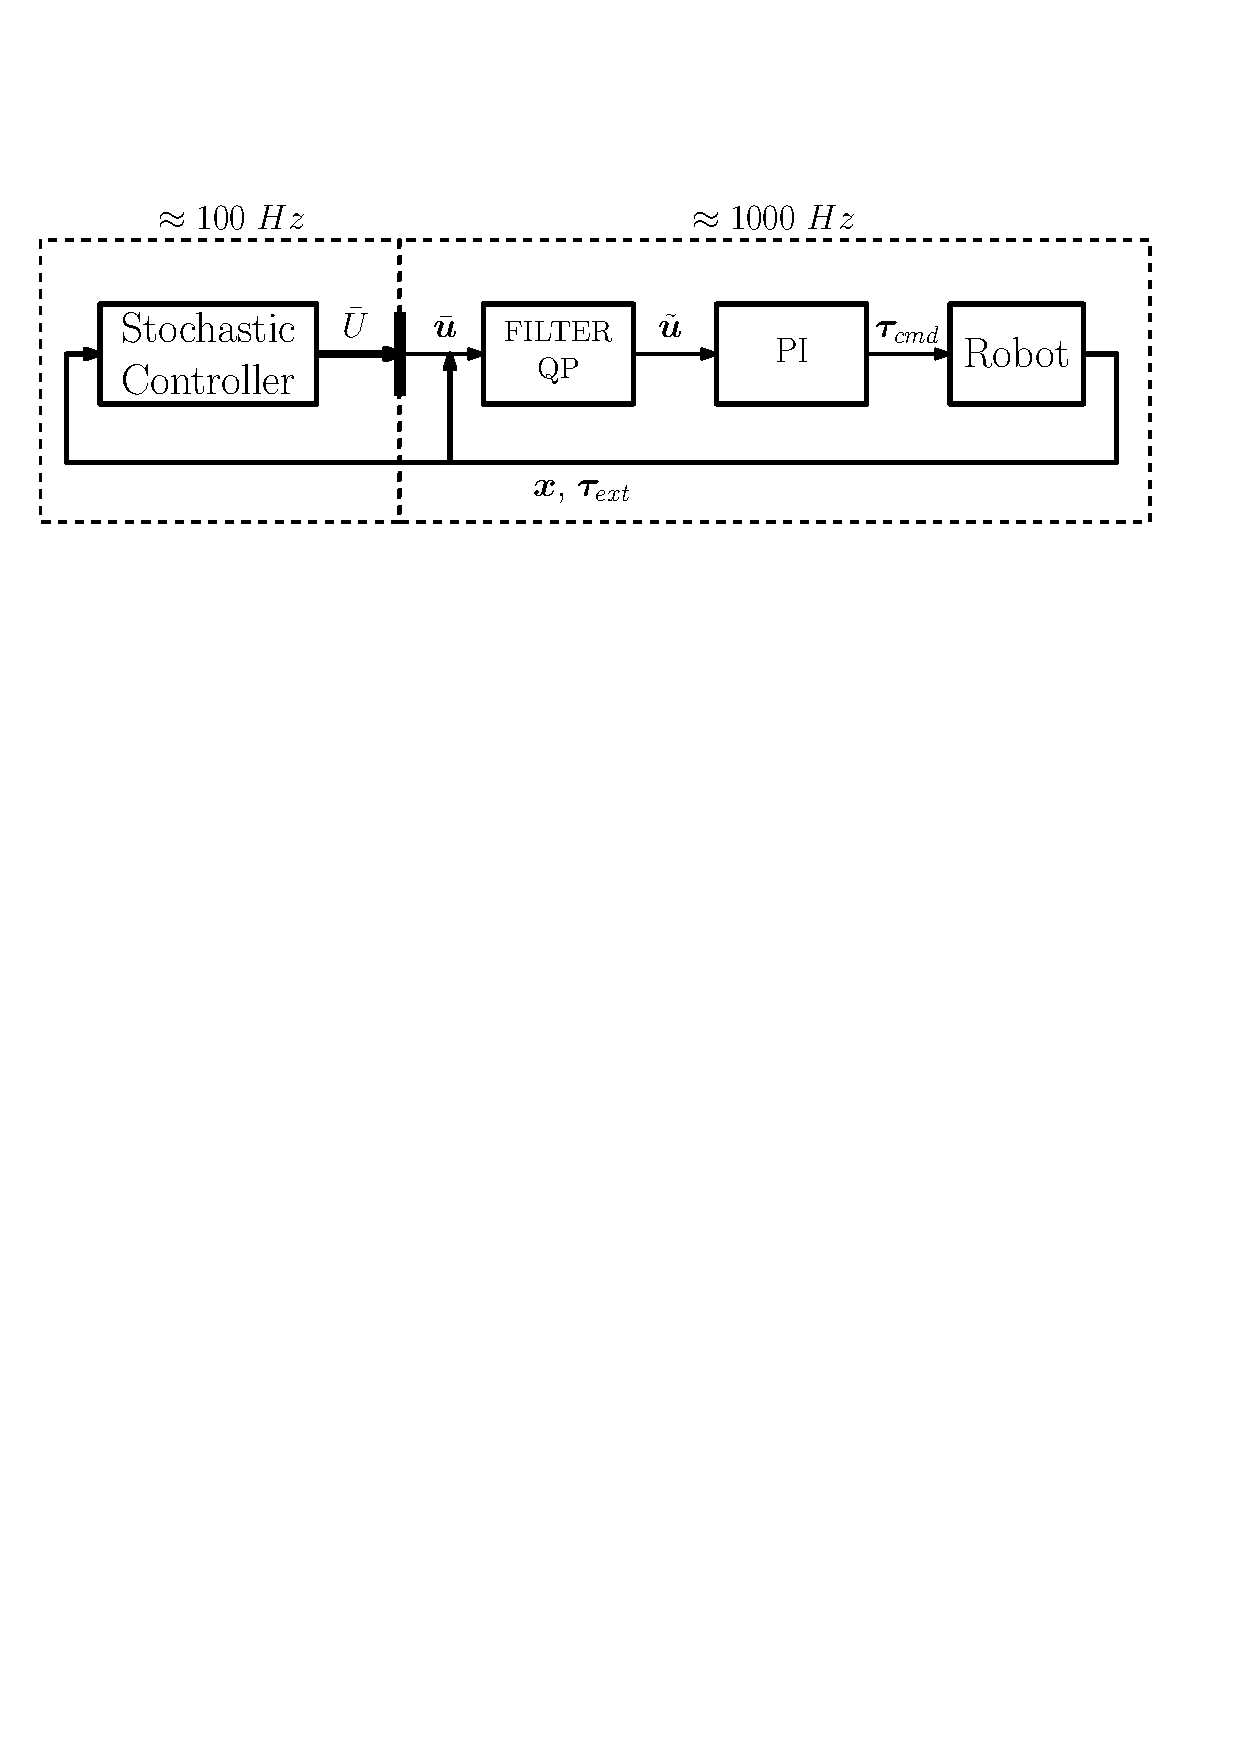
\includegraphics[width=1.1\columnwidth]{figures/schemes/high_level_architecture.pdf}
\caption{Cascaded control architecture: the sampling based controller computes a velocity trajectory $\bar{U}$ at approximately 100Hz. The input vector is queried and interpolated at a higher rate of approximately 1000Hz (tick line) and is filtered using the latest odometry.} \label{fig:cascaded_architecture}
\end{figure}

We can now summarize as follows all the possible approaches to the mobile manipulation control problem. We denote each controller with $\Pi_{*}$ where $*$ can be $N,\ O,\ I,\ IO$:
\begin{itemize}
    \item[$\Pi_{N}$:] relies exclusively on a stochastic controller to generate velocity commands, namely the input is not filtered either by a FILTER-QP or a Sequential FILTER-QP
    \item[$\Pi_{O}$:] a FILTER-QP is used to optimize the input sequence received by the stochastic controller. The FILTER-QP is solved at the same rate as the low-level controller,
    \item[$\Pi_{I}$:] the Sequential FILTER-QP is used in the stochastic controller to enforce safety and passivity constraints  as described in \algo \ref{algo:sequential_qp}. No FILTER-QP is solved at higher rate in the low-level controller.
    \item[$\Pi_{IO}$:] the full cascaded architecture (see \fig \ref{fig:cascaded_architecture}) is deployed, combining the previous two methods.
\end{itemize}
